\documentclass[10pt,journal,compsoc]{styles/IEEEtran}
\usepackage{styles/algorithm}
\usepackage[noend]{styles/algorithmic}
\usepackage{graphicx}
\usepackage{color}
\usepackage{listings}
\usepackage{amsmath}
\usepackage[utf8]{inputenc}
\usepackage[T1]{fontenc}
\usepackage[labelformat=empty]{caption}
% *** CITATION PACKAGES ***
\ifCLASSOPTIONcompsoc
  % IEEE Computer Society needs nocompress option
  % requires cite.sty v4.0 or later (November 2003)
  \usepackage[noadjust]{cite}
\else
  % normal IEEE
  \usepackage{cite}
\fi

\title{Tarea 8: Problemas de M\'inimos Cuadrados No Lineales}

\author{Juan Gerardo Fuentes Almeida}

% The paper headers
\markboth{Tarea 8: M\'inimos Cuadrados No Lineales}%
{Shell \MakeLowercase{\textit{et al.}}: Bare Advanced Demo of styles/IEEEtran.cls for Journals}

\IEEEtitleabstractindextext{%
\begin{abstract}
En esta pr\'actica se implementan los algoritmos de Gauss-Newton y Levenberg-Maquardt para resolver problemas de optimización con Mínimos Cuadrados No Lineales, aplicados a desenvolvimiento de fases.
\end{abstract}
}

\begin{document}

% make the title area
\maketitle

\IEEEdisplaynontitleabstractindextext

\IEEEpeerreviewmaketitle

\section{Introducci\'on}

\IEEEPARstart{E}n Problemas de Mínimos Cuadrados, la función objetivo $f$ tiene la forma especial:\\
 
 $f(x)=\frac{1}{2} \sum \limits_{j=1}^{m} r^2_j (x)$\\
 
donde cada $r_j$ es una función residual suave de $\Re^n$ a $\Re$, esta forma especial hace que el problema sea mas fácil de resolver comparado con un problema general de optimización sin restricciones.\\

Ensamblamos los componentes individuales de $r_j$ en un vector residual $r:\Re^n \rightarrow \Re^m$, de la siguiente manera:\\

$r(x)=(r_1(x),r_2(x),...,r_m(x))^T$\\

Con esta notación, podemos reescribir $f$ como $f(x)=\frac{1}{2} \parallel r^2_j (x) \parallel _2^2$, y sus derivadas en términos del Jacobiano $J(x)$:\\

\begin{figure}[hbtp]
\centering
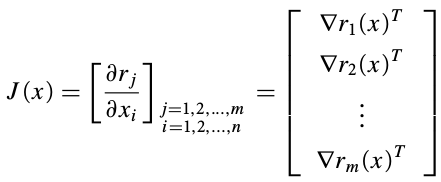
\includegraphics[width=0.35\textwidth]{Jacobian.png}
\caption*{}
\end{figure}

El gradiente y el Hessiano de $f$ se pueden expresar de la siguiente manera:\\

\begin{figure}[hbtp]
\centering
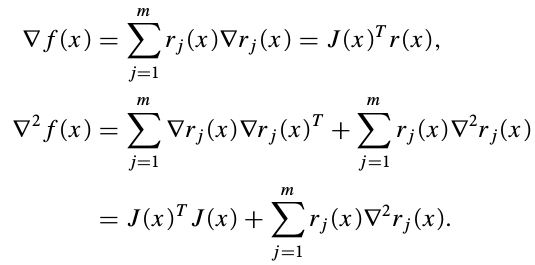
\includegraphics[width=0.4\textwidth]{Hessian.png}
\caption*{}
\end{figure}

En muchas aplicaciones, las primeras derivadas parciales de los residuales, y por tanto, de la Matriz Jacobiana $J(x)$ son relativamente fáciles de calcular. Asimismo, utilizando $J(x)$ podemos calcular el primer t\'ermino $J(x)^T J(x)$ del Hessiano sin evaluar las segundas derivadas de la función $r(x)$, esto es distintivo de los problemas de mínimos cuadrados, ya que los residuos $r_j$ están cerca de la solución, y por tanto, $\nabla^2 r_j (x)$ es relativamente pequeño.\\

\section{Teoría}

\subsection{M\'etodo de Gauss-Newton}

Puede verse como un método de Newton modificado con una búsqueda en linea, en el cual se resuelve el siguiente sistema para obtener la dirección de búsqueda $p_k$:\\

$J_k^T J_k p_k^{GN}=-J_k^{T} r_k$\\

Este método simplifica el tiempo de c\'alculo aproximando $\nabla ^2 f_k$ mediante el producto $J_k^T J_k$; \'este t\'ermino dominante mantiene un tiempo de convergencia cercano al del método de Newton. Además, $p_k^{GN}$ es una dirección de descenso si $J(x)$ tiene rango completo y $\nabla f_k$ es diferente de cero.\\

\subsection{M\'etodo de Levenberg-Maquardt}

Este método, al igual que el de Gauss-Newton utiliza la misma aproximación del Hessiano, pero reemplazando la búsqueda en linea con una estrategia de región de confianza, evitando que el sistema tenga un rango deficiente, como puede ocurrir en el método de Gauss-Newton, al mismo tiempo que mantiene también propiedades de convergencia similares. En este método se resuelve un sistema de ecuaciones de la forma:\\

$(J_k^T J_k+\lambda I)p_k^{LM}=-J_k^T r_k$\\

para un escalar $\lambda$, en \'esta implementación se propone un valor mayor al eigenvalor m\'as pequeño de la matriz $J_k^T J_k$.\\

\section{Implementaci\'on}

Sea $f(x)$ la fase desenvuelta de una imagen, y $g(x)$ su fase envuelta, por la propiedad de Nyquist, si la derivada de una función esta acotada en $(-\pi,\pi)$, es decir, $f(x)-f(x-e_1) \in (-\pi,\pi)$, entonces:\\

$f(x)-f(y)=W[g(x)-q(y)]$\\

siendo $W$ el operador de envolvimiento y $\parallel y-x \parallel=1$\\

luego, para recuperar $f(x)$ de $g(x)$, calculamos:\\

$g'_1(x)=g(x)-g(x-e_1)$, $g'_2(x)=g(x)-g(x-e_2)$\\

y envolvemos la función resultante:\\

$\widehat{g'_1(x)}=W[g'_1(x)]$, $\widehat{g'_2(x)}=W[g'_2(x)]$\\

Por tanto, por el criterio de Nyquist, podemos aproximar el residuo entre esta función y la derivada de la fase desenvuelta mediante mínimos cuadrados:\\

$U(f)=\sum \limits_{\Omega} [\widehat{g'_1(x)}-f'_1(x)]^2+\sum \limits_{\Omega} [\widehat{g'_2(x)}-f'_2(x)]^2$\\

donde $f'_1(x)=f(x)-f(x-e_1)$ y $f'_2(x)=f(x)-f(x-e_2)$ son las derivadas de la fase desenvuelta, las cuales podemos aproximar mediante Bases de Funciones Radiales:\\

$f(x)=\sum \limits_{ij} \alpha_{ij} \phi(i,j,x)$

con $\phi(i,j,x)=\exp[\frac{-1}{2\sigma_{ij}}(x-\mu_{ij})^2]$\\

luego\\
$f'_1(x)=\sum \limits_{ij}\alpha_{ij}[\phi(i,j,x)-\phi(i,j,x-e_1)]=\sum \limits_{ij}\alpha_{ij}\varphi_1 (i,j,x)$\\
y $f'_2(x)=\sum \limits_{ij}\alpha_{ij}[\phi(i,j,x)-\phi(i,j,x-e_2)]=\sum \limits_{ij}\alpha_{ij}\varphi_2 (i,j,x)$\\

luego, para recuperar $f(x)$ de $g(x)$, tendremos que minimizar la siguiente expresión:\\

$U(f)=\sum \limits_{\Omega} [\widehat{g'_1(x)}-f'_1(x)]^2+\sum \limits_{\Omega} [\widehat{g'_2(x)}-f'_2(x)]^2$\\

\subsection{Optimización de $\alpha$}

Para optimizar el valor de $\alpha$, el cual es la amplitud de las funciones radiales, se construye un Jacobiano cuyas filas son los componentes en $x$ y en $y$ de la función objetivo (2 veces el numero de pixeles de la imagen)\\

\[J(\alpha)= \left( \begin{array}{cccc}
\frac{\partial r(x_1)}{\partial \alpha_1} & \frac{\partial r(x_1)}{\partial \alpha_2} & \ldots & \frac{\partial r(x_1)}{\partial \alpha_m} \\
\vdots & \vdots & \ddots & \vdots \\
\frac{\partial r(x_N)}{\partial \alpha_1} & \frac{\partial r(y_N)}{\partial \alpha_2} & \ldots & \frac{\partial r(x_N)}{\partial \alpha_m} \\
\frac{\partial r(y_1)}{\partial \alpha_1} & \frac{\partial r(y_1)}{\partial \alpha_2} & \ldots & \frac{\partial r(y_1)}{\partial \alpha_m} \\
\vdots & \vdots & \ddots & \vdots \\
\frac{\partial r(y_N)}{\partial \alpha_1} & \frac{\partial r(y_N)}{\partial \alpha_2} & \ldots & \frac{\partial r(y_N)}{\partial \alpha_m} 
\end{array} \right)\] 

El gradiente de la función esta determinado por $J_k^Tr_k$.\\

Cada elemento de esta matriz esta definido por la siguiente expresión:\\

$\frac{\partial r(x_k)}{\partial \alpha_{ij}}=-\varphi_1(i,j,x_k)=-\frac{(x_{k_1}-\mu_{ij_1})}{\sigma_{ij}^2}\phi(i,j,x_k)$\\

$\frac{\partial r(y_k)}{\partial \alpha_{ij}}=-\varphi_2(i,j,x_k)=-\frac{(x_{k_2}-\mu_{ij_2})}{\sigma_{ij}^2}\phi(i,j,x_k)$\\

\subsection{Optimización de $\mu$}

Para optimizar el valor de $\mu$, el cual es la media de las funciones radiales, se construye un Jacobiano cuyas filas son los componentes en $x$ y en $y$ de la función objetivo (2 veces el numero de pixeles de la imagen), y cuyas columnas están repartidas entre las componentes en x y en y de la medias (2 veces el numero de funciones radiales):\\

\[J(\mu)= \left( \begin{array}{cccccc}
\frac{\partial r(x_1)}{\partial \mu(x_1)} & \ldots & \frac{\partial r(x_1)}{\partial \mu(x_m)} & \frac{\partial r(x_1)}{\partial \mu(y_1)} & \ldots & \frac{\partial r(x_1)}{\partial \mu(x_m)} \\
\vdots & \ddots & \vdots & \vdots & \ddots & \vdots \\

\frac{\partial r(x_N)}{\partial \mu(x_1)} & \ldots & \frac{\partial r(x_N)}{\partial \mu(x_m)} & \frac{\partial r(x_N)}{\partial \mu(y_1)} & \ldots & \frac{\partial r(x_N)}{\partial \mu(x_m)} \\
\frac{\partial r(y_1)}{\partial \mu(x_1)} & \ldots & \frac{\partial r(y_1)}{\partial \mu(x_m)} & \frac{\partial r(y_1)}{\partial \mu(y_1)} & \ldots & \frac{\partial r(y_1)}{\partial \mu(x_m)} \\
\vdots & \ddots & \vdots & \vdots & \ddots & \vdots \\

\frac{\partial r(y_N)}{\partial \mu(x_1)} & \ldots & \frac{\partial r(y_N)}{\partial \mu(x_m)} & \frac{\partial r(y_N)}{\partial \mu(y_1)} & \ldots & \frac{\partial r(y_N)}{\partial \mu(x_m)}
\end{array} \right)\] 

El gradiente de la función esta determinado por $J_k^Tr_k$. 

Cada elemento de esta matriz esta definido por la siguiente expresión:\\

\small 
$\frac{\partial r(x_k)}{\partial \mu(x_{ij})}=- \alpha_{ij} \frac{\partial \varphi_1(i,j,x_k)}{\partial \mu(x_{ij})} =- \frac{\alpha_{ij}}{\sigma_{ij}^2}\phi(i,j,x_k)[1-\frac{(x_{k_1}-\mu_{ij_1})^2}{\sigma_{ij}^2}] $\\
\normalsize

$\frac{\partial r(x_k)}{\partial \mu(y_{ij})}= \frac{\alpha_{ij}}{\sigma_{ij}^4}\phi(i,j,x_k)(x_{k_1}-\mu_{ij_1})(x_{k_2}-\mu_{ij_2})$\\

$\frac{\partial r(y_k)}{\partial \mu(x_{ij})}=\frac{\alpha_{ij}}{\sigma_{ij}^4}\phi(i,j,x_k)(x_{k_1}-\mu_{ij_1})(x_{k_2}-\mu_{ij_2})$\\

\small 
$\frac{\partial r(y_k)}{\partial \mu(y_{ij})}=- \alpha_{ij} \frac{\partial \varphi_1(i,j,x_k)}{\partial \mu(y_{ij})} =- \frac{\alpha_{ij}}{\sigma_{ij}^2}\phi(i,j,x_k)[1-\frac{(x_{k_2}-\mu_{ij_2})^2}{\sigma_{ij}^2}] $\\
\normalsize

\subsection{Optimización de $\sigma$}

Para optimizar el valor de $\sigma$, el cual es la desviación estándar de las funciones radiales, se construye un Jacobiano cuyas filas son los componentes en $x$ y en $y$ de la función objetivo (2 veces el numero de pixeles de la imagen)\\

\[J(\alpha)= \left( \begin{array}{cccc}
\frac{\partial r(x_1)}{\partial \sigma_1} & \frac{\partial r(x_1)}{\partial \sigma_2} & \ldots & \frac{\partial r(x_1)}{\partial \sigma_m} \\
\vdots & \vdots & \ddots & \vdots \\
\frac{\partial r(x_N)}{\partial \sigma_1} & \frac{\partial r(y_N)}{\partial \sigma_2} & \ldots & \frac{\partial r(x_N)}{\partial \sigma_m} \\
\frac{\partial r(y_1)}{\partial \sigma_1} & \frac{\partial r(y_1)}{\partial \sigma_2} & \ldots & \frac{\partial r(y_1)}{\partial \sigma_m} \\
\vdots & \vdots & \ddots & \vdots \\
\frac{\partial r(y_N)}{\partial \sigma_1} & \frac{\partial r(y_N)}{\partial \sigma_2} & \ldots & \frac{\partial r(y_N)}{\partial \sigma_m} 
\end{array} \right)\] 

El gradiente de la función esta determinado por $J_k^Tr_k$. 

Cada elemento de esta matriz esta definido por la siguiente expresión:\\

$\frac{\partial r(x_k)}{\partial \sigma_{ij}}=-\frac{\alpha_{ij}}{\sigma_{ij}^3}(x_{k_1}-\mu_{ij_1})\phi(i,j,x_k)[2-\frac{(x_k-\mu_{ij})^2}{\sigma_{ij}}]$\\

$\frac{\partial r(y_k)}{\partial \sigma_{ij}}=-\frac{\alpha_{ij}}{\sigma_{ij}^3}(x_{k_2}-\mu_{ij_2})\phi(i,j,x_k)[2-\frac{(x_k-\mu_{ij})^2}{\sigma_{ij}}]$\\

\section{Resultados}

A continuación se muestran las imágenes que se obtuvieron durante la ejecución de la práctica, para diferente n\'umero de funciones radiales en una imagen de prueba, utilizando los métodos de Gauss-Newton y Levenberg-Maquardt:\\


\begin{figure}[H]
\centering

\includegraphics[width=0.25\textwidth]{phase.png}
\caption{Imagen Desenvuelta}
\end{figure}

Los siguientes resultados fueron obtenidos con el método de Gauss-Newton:\\

\begin{figure}[H]
	\centering
	
\includegraphics[width=0.20\textwidth]{GN1_0.png}
	
\includegraphics[width=0.20\textwidth]{GN1_20.png}
	\caption{Der. a izq.: Imagen Inicial con 1 RBF, Después de 20 iteraciones}
\end{figure}

\begin{figure}[H]
	\centering
	
\includegraphics[width=0.20\textwidth]{GN2_0.png}
	
\includegraphics[width=0.20\textwidth]{GN2_20.png}
	\caption{Der. a izq.: Imagen Inicial con 2 RBF, Después de 20 iteraciones}
\end{figure}

\begin{figure}[H]
	\centering
	
\includegraphics[width=0.20\textwidth]{GN3_0.png}
	
\includegraphics[width=0.20\textwidth]{GN3_20.png}
	\caption{Der. a izq.: Imagen Inicial con 3 RBF, Después de 20 iteraciones}
\end{figure}

\begin{figure}[H]
	\centering
	
\includegraphics[width=0.20\textwidth]{GN4_0.png}
	
\includegraphics[width=0.20\textwidth]{GN4_20.png}
	\caption{Der. a izq.: Imagen Inicial con 4 RBF, Después de 20 iteraciones}
\end{figure}

\begin{figure}[H]
	\centering
	
\includegraphics[width=0.20\textwidth]{GN10_0.png}
	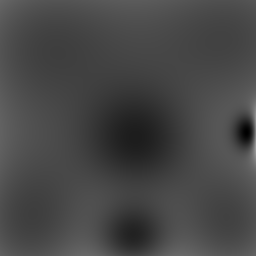
\includegraphics[width=0.20\textwidth]{GN10_20.png}
	\caption{Der. a izq.: Imagen Inicial con 10 RBF, Después de 20 iteraciones}
\end{figure}

La siguiente tabla muestra el desempeño de los algoritmos implementados en esta pr\'actica, para diferente numero de RBF's, como se observa, el comportamiento de ambos algoritmos es muy similar:

\begin{figure}[H]
\centering
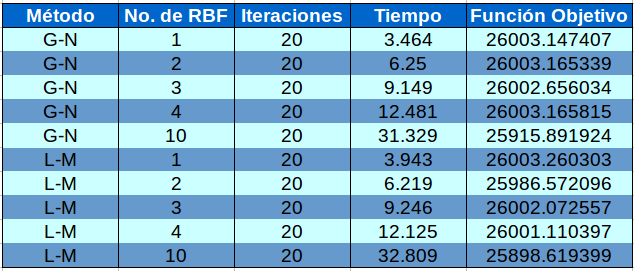
\includegraphics[width=0.5\textwidth]{tabla.png}
\caption{Desempeño de los métodos Gauss-Newton (G-N) y Levenberg-Maquardt (L-M)}
\end{figure}

\section{Conclusiones}

Cabe se\~nalar que como el inicio del algoritmo es estocástico, conviene correr el programa varias veces para obtener un resultado deseable, y como es de esperarse, cuantas m\'as señales gaussianas haya, le cuesta m\'as trabajo al algoritmo optimizar la función objetivo, aunque se observa que el algoritmo sigue un patrón: se coloca una gaussiana en el centro y las dem\'as en los bordes, comúnmente en las esquinas y sobre el punto medio de los lados, después de esto, se procede a disminuir el tamaño de las gaussianas en los bordes y a aumentar el tamaño de la gaussiana en el centro, basta con correr el algoritmo varias veces para un n\'umero grande de gaussianas (aprox. 10) para apreciar este comportamiento.\\

Otro detalle que se observ\'o, fue que en ocasiones el resultado se asemeja al que se muestra en la siguiente figura:\\

\begin{figure}[H]
\centering
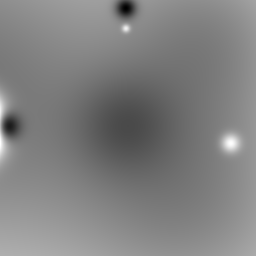
\includegraphics[width=0.25\textwidth]{case.png}
\caption*{}
\end{figure}

Este resultado no necesariamente es erróneo, ya que debemos considerar que la normalización de la imagen altera la percepción de las intensidades, en esta imagen se aprecia que los puntos muy negros de la parte superior y de la izquierda tienen impacto sobre la normalización de los pixeles de la imagen, considerando también que el resultado de la función objetivo para este caso fue similar a los otros resultados mostrados en las imágenes anteriores; la mancha semi-oscura del centro muestra que el algoritmo si trat\'o de realizar la optimización, aunque la parte de la optimización de las medias no fue suficientemente eficiente para desplazar las señales indeseables hacia afuera de la imagen.\\ 

\bibliographystyle{plain}
\bibliography{biblio}


\appendix
\section{Implementation details}
El programa est\'a implementado tomando en cuenta todas estandarizaciones indicadas en el curso.

El \textit{makefile} que se ha generado, incluye los comandos \textit{make}, \textit{run}, \textit{test} y \textit{clean}. El programa recibe el nombre del archivo de la imagen y el parámetro \textit{methodID}, el cual indica al programa que método de optimización se va a usar, 1 para Gauss-Newton y 2 para Levenberg-Maquardt, el comando \textit{test} ejecuta 20 iteraciones del método de Gauss-Newton con 1 gaussiana.\\

\begin{figure}[H]
\centering
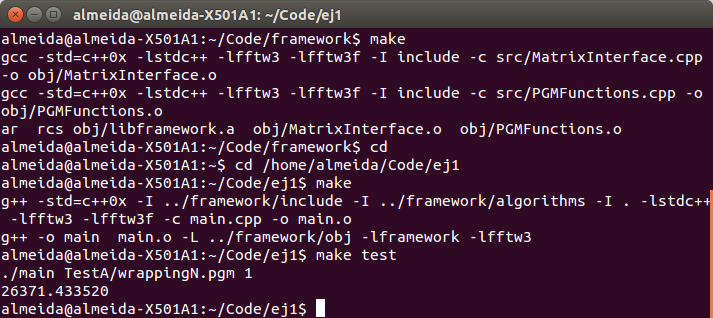
\includegraphics[width=0.5\textwidth]{screen.png}
\caption*{}
\end{figure}

\end{document}


